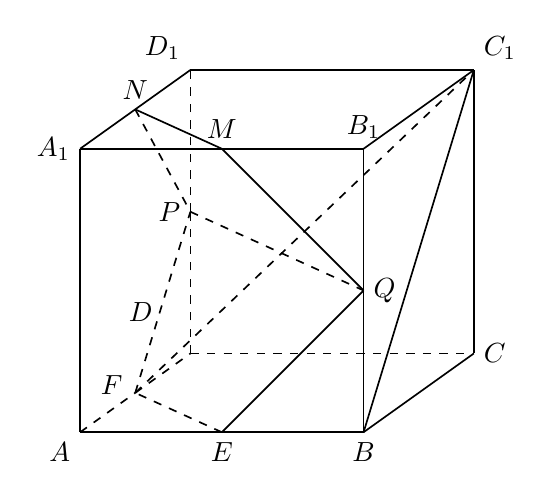
\begin{tikzpicture}[x=1cm,y=1cm,line width=0.6pt,font=\normalsize]
\coordinate (A) at (0,0);
\coordinate (B) at (3.6,0);
\coordinate (B1) at (3.6,3.6);
\coordinate (A1) at (0,3.6);
\coordinate (D) at (1.4,1.0);
\coordinate (C) at (5.0,1.0);
\coordinate (D1) at (1.4,4.6);
\coordinate (C1) at (5.0,4.6);
\coordinate (E) at (1.8,0);
\coordinate (F) at (0.7,0.5);
\coordinate (P) at (1.4,2.8);
\coordinate (Q) at (3.6,1.8);
\coordinate (M) at (1.8,3.6);
\coordinate (N) at (0.7,4.1);
% front face solid
\draw[solid] (A)--(E);
\draw[solid] (E)--(B);
\draw[solid] (B)--(Q);
\draw[solid] (Q)--(B1);
\draw[solid] (B1)--(M);
\draw[solid] (M)--(A1);
\draw[solid] (A1)--(A);
% top/back visible solid
\draw[solid] (D1)--(C1);
\draw[solid] (A1)--(N);
\draw[solid] (N)--(D1);
\draw[solid] (C1)--(C);\draw[solid] (B)--(C);
% section EFPQ: E-Q solid, rest dashed
\draw[solid] (E)--(Q);
\draw[dashed] (E)--(F);
\draw[dashed] (F)--(P);\draw[dashed] (F)--(C1);
\draw[dashed] (P)--(Q);
% section PQMN: N-M and M-Q solid, rest dashed
\draw[solid] (N)--(M);
\draw[solid] (M)--(Q);
\draw[dashed] (N)--(P);
% diagonal BC1 solid
\draw[solid] (B)--(C1);
% hidden cube edges
\draw[dashed] (A)--(F);
\draw[dashed] (F)--(D);
\draw[dashed] (D)--(C);
\draw[dashed] (D)--(P);
\draw[dashed] (P)--(D1);
\draw[solid] (B1)--(C1);
% labels
\node[below left] at (A) {$A$};
\node[below] at (E) {$E$};
\node[below] at (B) {$B$};
\node[left,xshift=-1.0pt,yshift=3.0pt] at (F) {$F$};
\node[above left=3pt,xshift=-7pt,yshift=5pt] at (D) {$D$};
\node[right] at (C) {$C$};
\node[left] at (A1) {$A_{1}$};
\node[above] at (N) {$N$};
\node[above left] at (D1) {$D_{1}$};
\node[above] at (M) {$M$};
\node[above] at (B1) {$B_{1}$};
\node[above right] at (C1) {$C_{1}$};
\node[left] at (P) {$P$};
\node[right] at (Q) {$Q$};
\end{tikzpicture}
